\chapter{Stand der Forschung}

Im folgenden Kapitel wird ein grundlegendes Verständnis für die Funktionsweise von Strukturbatterien vermittelt. Außerdem werden die Besonderheiten im Vergleich zu konventionellen Batterien und faserverstärkten Verbundwerkstoffen erläutert. Dazu werden die wichtigsten Eigenschaften und deren Ermittlungsverfahren dargestellt sowie die Rolle der einzelnen Komponenten im Zusammenhang mit der Materialauswahl näher erklärt. Anschließend werden aktuelle Entwicklungsansätze diskutiert und abschließend die ungelösten Herausforderungen mit den aktuellen Methoden näher analysiert.

\section{Funktionsweise der Strukturbatterie} Strukturbatterien sind Batterien, die mechanisch belastbar sind und damit auch zur strukturellen Integrität beitragen können.
Batterien erlauben es, temporär Energie zu speichern, indem Ladungsträger reversibel in einem Hostmaterial eingelagert werden. Solche Zellen werden daher auch ''Shuttle-Clock''\cite{Ohzuku1993}-, ''Rocking-Chair''\cite{Tarascon1993}- oder ''Swing''\cite{Bittihn1993}-Zellen genannt. Der Einlagerungsprozess selbst wird meist als ''Interkalation'' bezeichnet \cite{Eichinger1976}. Durch den Einlagerungsprozess nehmen die beiden Hostmaterialien aktiv am Ladungsaustausch teil, daher auch der Name ''Aktivmaterial'', siehe Bild~\ref{fig:battery_function}. Häufig ist das Aktivmaterial für die Anode Graphit und für die Kathode ein Metalloxid (\ce{MO_2}).
\begin{figure}[h]
	%\raggedleft
		%\def\svgwidth{\columnwidth}
        \center
	\includegraphics[width=\textwidth, angle=0]{battery_function.pdf}
		\caption{\label{fig:battery_function}Die Energiespeicherfunktion einer Batterie wird maßgeblich durch den skalenübergreifenen Ein- und Auslagerungsprozess der Ladungsträger realisiert.}
\end{figure}
Beim Entladen der Batteriezelle wandern die Ladungsträger von der Anode zur Kathode. An beiden Elektroden kommt es zum Ladungsaustausch, der mittels Redox-Gleichungen beschrieben werden kann \cite{Goodenough2013}: 
\begin{align}
	\ce{C_6 + x Li^+ + x e^- &<=> Li_xC_6}\\ 
	\ce{LiMO_2 - x Li^+ - x e^- &<=> Li_{1-x}MO_2} 
\end{align} 
Der Einlagerungsprozess erlaubt im Vergleich zur reinen elektrostatischen Speicherung, wie etwa bei Kondensatoren, eine signifikant höhere Beladungsdichte an Ladungsträgern, wodurch größere Energiemengen gespeichert werden können.

Entscheidend für die Funktion der Batterie ist hierbei, dass der Transport der Ionen durch den Elektrolyten und den Separator erfolgt. Die Elektronen können jedoch nur entlang des Stromkollektors geleitet werden und müssen daher einen „Umweg“ außerhalb der Zelle machen, siehe Bild~\ref{fig:battery_function}. Die Bewegung der Elektronen ist dabei im Vergleich zum Ionentransport deutlich schneller, weshalb die Ent- und Beladungsgeschwindigkeit einzig von der Ionenmobilität limitiert wird.

Im Falle großer Ströme, wie etwa bei einem Kurzschluss, finden viele Ladungsumwandlungsreaktionen gleichzeitig statt. Die dabei entstehende Wärme kann zum Versagen oder Brennen der Zelle führen. Mögliche Ursachen für Kurzschlüsse sind Herstellungsfehler, Dendritwachstum und mechanische Belastungen, bei denen die Elektroden durch Versagen des Separators in direkten Kontakt kommen, wie etwa bei Penetration oder Biegung.

Darüber hinaus führt die mit den mechanischen Belastungen einhergehende Rissbildung zu einer Erhöhung des inneren elektrischen Widerstandes, was zu einem Verlust an Speichereffizienz führt und daher vermieden werden soll. Bei konventionellen Batterien kommen daher spezielle Umhausungen zum Einsatz, die eine Belastung der Batterien verhindern sollen. Diese bringen allerdings einen signifikanten Anteil an zusätzlicher Masse hinzu und sind aufgrund ihrer Größe meist schwerer in Hoststrukturen zu integrieren. Um diesen Nachteilen zu begegnen, versuchen Strukturbatterien durch die Integration geeigneter Materialien die mechanische Belastungsfähigkeit zu verbessern. Zur Steigerung der Multifunktionalität neuer Strukturbatterien ist daher neben einem umfangreichen Verständnis der wichtigsten Eigenschaften auch ein Überblick über mögliche Materialkandidaten aus bestehenden Untersuchungen zu konventionellen Batterien sowie dem Leichtbaubereich notwendig.


\section{Wichtigsten Eigenschaften und ihre Ermittlungsverfahren}
%\subsection{Interkalation}
\subsection{Ladungszustand}
Ein wesentliches Merkmal von Batterien ist die Einlagerung von Ionen in das Hostmaterial (Interkalation). Je nach Hostmaterial stehen dabei eine bestimmte Menge an Einlagerungsplätzen zur Verfügung. Der Ladungszustand (\textit{engl.} state of charge) beschreibt dabei den Anteil von besetzen Plätzen zu insgesamt verfügbaren Plätzen.
Dies bedeutet, dass wenn alle Plätze belegt sind SoC=1 oder 100~\% ist und falls alle Ionen das Hostmaterial verlassen haben, also keiner der Plätze belegt ist, SOC einen Wert von 0~\% hat.
Der SOC hat maßgeblich Wirkungen auf das chemische Potenzial und die Diffusionsgeschwindigkeiten. Der SOC kann jedoch nicht direkt gemessen werden und wird über die Elektrodenspannung ermittelt.
\begin{table}[ht]
    \centering
    \caption{\label{tab:volume_change}Volumenänderungen bo der Lithiierung für gängige Aktivmaterialien.}
    \begin{tabular}[t]{lccc}
        \toprule
        Material& Volumenänderung $\Delta$V/V\textsubscript{0}&Verlauf&Referenz\\
        \midrule
        Graphit & +10\% - +13\% & nicht-linear & \cite{Qi2010,Woodford2012}\\
        NMC111 &-2,4\%&nicht-linear& \cite{Yabuuchi2005}\\
        NMC422 &+2,4\%&nicht-linear& \cite{Ma2007}\\
        LCO &-1,9\% & linear & \cite{Reimers1992}\\
        NCA &-1,6\% & nicht-linear& \cite{Itou2005}\\
        LFP &+6,5\% & linear & \cite{Padhi1997}\\
        LMO &+6,6\% & linear & \cite{Christensen2006}\\
        \bottomrule
    \end{tabular}
\end{table}

\subsection{Elektrische Spannung}

Die elektrische Spannung ist neben dem Strom, der direkt mit der Bewegung der Ladungsträger gekommt ist einer der wichtigsten Größen zur beschreibung des Zustandes in einer Batteriezelle. 

Die Leerlaufspannung wird gemessen, wenn kein Strom zwischen den zwei Elektroden fließt und ist damit entscheident für die Beschreibung des Gleichgewichtszustandes innerhalb der Zelle.
Allgemein sinkt die Spannung mit steigender Entladung der Elektrode. Abhängig von der chemischen Striktur variert das Einalgerungsverhalten, was in den Kurvenanstiegen bemerkbar macht.
Die Spannung der Batterie ist dabei die Differenz der beiden Referenzspannungen.
Zwei der wichtigsten Spannungsgrößen einer Batterie ist die nominale Spannung und die Abschaltspannung, die die minimal erlaubte Spannung und damit den ''entladenen'' Zustand markiert.

\begin{figure}[h]
	%\raggedleft
		%\def\svgwidth{\columnwidth}
        \center
	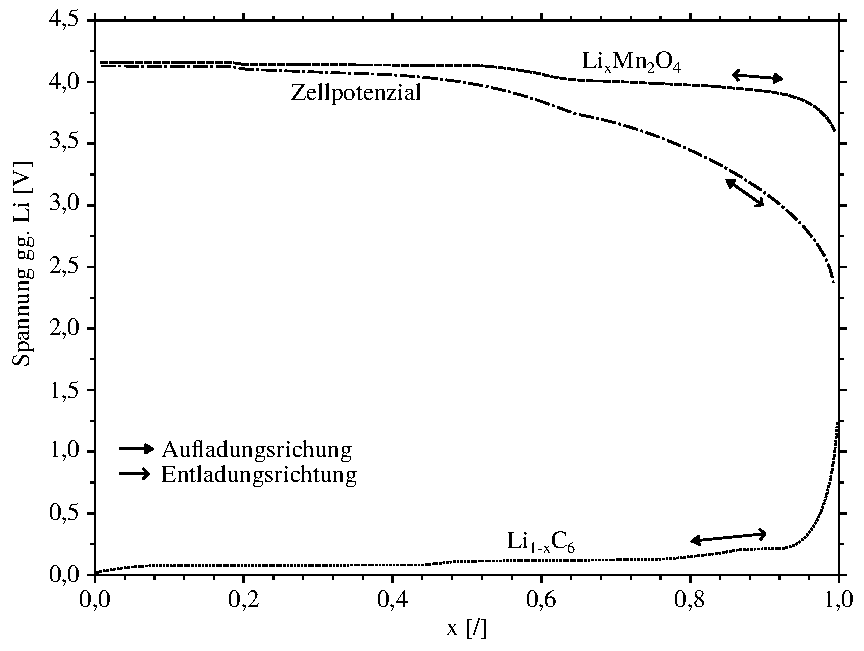
\includegraphics[width=\textwidth, angle=0]{uocp.pdf}
		\caption{\label{fig:battery_voltage}Spannung über den stöchiometrischen Anteil der beladung einer Lithiumionenbatterie, sowie die Anteile der negativen (Graphit) und positiven (Manganoxid) Elektrode (angelehnt an~\cite{Newman2021}).}
\end{figure}

\subsection{C-Raten}
Die Auflade- oder Entladerate einer Batterie wird oft in sogenannten C-Raten angegeben. Dabei meint 1~C, dass eine voll entladene/beladene Batterie in 1~h komplett aufgeladen/entladen wird. Bei einer doppelt so hohen C-Rate wird die Batterie folglich in halber Zeit also 30~min entladen bzw. aufgeladen. Bei einer halb so hohen Auflade- bzw. Entladerate (0.5C oder C/2) benötigt die Batterie 2~h um komplett aufgeladen oder entladen zu werden.
Die Wahl der C-Rate ist vor allem bei der Messung von Kapazität von Bedeutung.
Verallgemeinert gilt, je höher die C-Rate desto geringer ist die gemessene Kapazität. Die Stärke des Kapazitätsabfalls wird durch eine Reihe wie Faktoren, wie Übergangsverhalten, Form und Art der chemischen Struktur der Elektrode usw. bestimmt.

\subsection{Kapazität}
Die Kapazität einer Elektrode beschreibt wie viele Ladungsträger eingelagert oder entfernt werden konnten. Besonders in den ersten Zyklen ist der Unterschied zwischen Auflade- ($\text{C}_{\text{aufl}}$) und Entladekapazität ($\text{C}_{\text{entl}}$) signifikant, weshalb die Kapazität für beide Prozesse getrennt bestimmt wird.

Zur Ermittlung der Kapazität wird konstanten Auflade- ($\text{I}_\text{C,aufl})$ oder Entladestrom ($\text{I}_\text{C,entl})$ (C-Rate) an eine Zelle aus Elektrode und Referenzelektrode, meist Lithiummetall, angelegt und die Zeit $\Delta \text{T}_\text{aufl}$ gemessen die für die komplette Auf- bzw. Entladung benötigt wird. Da die Kapazität das zeitliche Integral des Stromes ist, kann die bestimmung zu den folgenden Formeln vereinfacht werden
\begin{align}
	\text{C}_{\text{aufl}} &= \text{I}_\text{C,aufl} \cdot \Delta \text{T}_\text{aufl}\\
	\text{C}_{\text{entl}} &= \text{I}_\text{C,entl} \cdot \Delta \text{T}_\text{entl}.
\end{align}

%komplett entladen oder in der die Spannung von Abschalt- bzw. Leerspannung $\text{U}_{\text{leer}}$ zur vorher ermittelten maximal Spannung $\text{U}_{\text{voll}}$ benötigt. Die Aufladekapazit stellt dabei das Produkt aus Durch Umkehrung des Prozesses lässt sich die Entladekapazität bestimmen 

Bei der Entwicklung neuer Batteriematerialien wird die Kapazität meist auf die Masse des am Einlagerungsprozess teilnehmenden Material (Aktivmaterial) normiert. Diese spezifische Kapazität hat dann die Einheit [$\si{\A \hour \per \g}$]. Im Kontext der Batterieentwicklung wird allerdings die Kapazität je Elektrodenfläche [$\si{\A \hour \per \cm \squared}$] häufig angegeben.


\subsection{Columbische Effizienz}
Die Coulumbische Effizienz (CE) ist eienr der meist benutzen Metriken um die intern Reaktion die eine. Die CE vom Zyklus n ist definiert als das Verhältnis der gemessene Kapazität während des Entladevorgangs $C_{Dch}(n)$ zum Kapaziät des vorherigen Beladungsvorganges $C_{Ch}(n)$ \cite{Tornheim2020}.
Die Formel
\begin{equation}
CE = \frac{C_{Dch}(n)}{C_{Ch}(n)}
\end{equation}
gilt dabei für Aufbauten, die in einem Entladenzustand zusammengebaut werden und daher zu erst Beladen werden müssen. Zellen die in einem beladenen Zustand gefertigt werden, wie etwa Lithium-Schwefel-Batterien beginnen allerdings zu erst mit einem Entladungszyklus. Die korrekte Formel lautet in einem solchen Fall
\begin{equation}
    CE = \frac{C_{Dch}(n+1)}{C_{Ch}(n)}.
\end{equation}

\subsection{Kapaziätserhalt}
Die Kapaziätserhalt (\textit{engl.} Capacity Retention) ist eine wichtige Metrik um den Anteil an Nebenreaktionen die zu einem Kaparzitätsverlust in Batterien führen zu bemessen. Sie ist definiert als das Verhältnis von Entladungskapazität des n+1 zykluses $C_{Dch}(n+1)$ und der des n-ten Zyklus $C_{Dch}(n)$ 
\begin{equation}
    CE = \frac{C_{Dch}(n+1)}{C_{Ch}(n)}.
\end{equation}
In einigen Fällen wird CR auch im Verhältnis zur intiiallen Entlade Kapazität bestimmt, also
\begin{equation}
    CE = \frac{C_{Dch}(n)}{C_{Ch}(1)}.
\end{equation}
Dieser Ansatz ist besonders dann hilfreich wenn die Langlebigkeit zu bestimmen \cite{Tornheim2020}.
Im Gegensatz zu CE ist CR meist relevanter Hersteller und Endnutzer.



\subsection{Energiedichte}
Die gravimetrische oder volumetrische Energiedichte ist eine der wichtigsten Metriken für Batterien. Sie gibt an wie viel Energie relative zur Masse oder Volumen gespeichert werden kann. 

Einer der größten Schwierigkeiten beim Umgang mit angebenen Energiedichten aus der Literatur besteht in dem Umstand, dass oft bei der Masse oder Volumen sich auf verschiedene Komponenten bezogen wird. Im allgemeinen Unterscheidet die Angaben ob die Werte im Kontext von:
\begin{enumerate}
	\item Materialentwicklung
	\item Elektrodentwicklung
	\item Zellentwicklung
\end{enumerate}
erhoben wurden \cite{Son2021}.
So wird bei der Forschung von neuen Aktivmaterialien, die spezifische Energie pro eingesetzte Masse an Aktivmaterial bezogen. Bei der 

%\subsection{Zyklenverhalten}
\subsection{Steifigkeit und Festigkeit}
%\subsection{Mechanische Spannung}
\subsection{Multifunktionale Effizienz}

Die einheitenlose multifunktionale Effizienz ist ein Maß um zu bewerten ob ein Vorteil durch den Einsatz von multifunktionalen Lösungen gegenüber einem kombinierten Einsatz von monofunktionalen Komponenten entsteht.
Die multifunktionale Effizienz wurde erstmalig von XXX eingeführt und ist die Summe der mechanischen  und elektrochemsichen Effizienz.
\begin{align}
	\eta_{\text{mutli}} &= \eta_{\text{mech}} + \eta_{\text{elchem}}\\
						&= \frac{E}{E_{\text{ref}}} + \frac{\Gamma}{\Gamma_\text{ref}} 
\end{align}
Im Kontext von Strukturspeicher wird für die mechanische Effizienz oft der das Verhältnis der spezifischen Steifigkeiten, oft das Elastizitätsmodul, der multifunktionalen Strukturbatterie und der eines UD-Kohlefasergeleges. Ähnlich ergibt sich elektrochemische Effizienz der Strukturbatterie aus dem Verhältnis der jeweiligen Energiedichten. Ein multifunktionaler Effizienzwert größer gleich eins Bedeutet damit, dass durch den Einsatz eine Reduktion der Gesamtmasse gegenüber der monofunktionalen Lösung besteht.

\section{Materialauswahl}

Jedes  Material in einer Strukturbatterie erfüllt mehrere Aufgaben gleichzeitig. Dies bedeutet, dass 
Die am meisten benutzte Untergliederung teilt die Materialien nach ihrer elektrochemischen Rolle ein.


\subsection{Anode}
Die Anode sollte ein niedriges elektrochemisches Potenzial und eine schnelle Interkalation für eine möglichst hohe Energiedicht und Leistungsdichte aufweisen. Zusätzlich profitieren Strukturbatterien sehr von Anoden mit hohen Festigkeits- und Steifigkeitswerten.

Die Verwendung von Kohlenstoff in Lithium-Ionen Batterien wurde erstmalig von \textsc{Yoshino} \cite{Yoshino1986} 1886 veröffentlicht der für diesen Durchbuch 2019 den Nobelpreis erhielt.
Heute ist Kohlenstoff eines der meist benutzen Material in wiederaufladbaren nicht-aqueous Batterien \cite{Ahmad2021}. Am meist verbreitesten ist dabei die Kombination von Grafit als Anode und einer Kathode aus Phosphat, welche eine maximale Energiedichte von 200-250~$\si{\watt \hour \per \kg}$. 
Es gibt zwei Arten von Kohlenstoff die in der Lage sind Ionen einzulagern: geordenten und ungeordenten \cite{Ghosh2024}.

Geordenter Kohlenstoff sind Materialien mit einer weitreichenden Ordnung ud hoger Kristallinität. Die Ordnung kann sich dabei auf eine Achse (CNTs), eine Ebene (Graphen) oder den Raum (Grafit) begrenzen \cite{Wang2021}.

Grafit hat eine hoch-kristaline Struktur und besitzt eine weit reichende Ordnung. Die $\text{sp}^\text{2}$-hybritisierten Graphenelagen sind in lang der c-Achse gestappelt und folgen entweder die hexagona AB-Sequenz oder dei rhombohedrale ABC-Folge. Die binden $\pi$-Orbitale ermögliche eine gute Leitfähigkeit von $10^3$-$10^4$~$\si{\siemens \per \cm}$ in Ebenenrichtung. Die Graphenebenen ahben einen Abstand von 3,35~$\si{\angstrom}$ entlang der c-Achse und werden nur durch relativ schwache van der Waals Kräfte (16-17~$\si{\kJ \per \mol}$) zusammen gehalten. Der relative hohe Abstand und die schwachen Bindungskräfte machen es einfach, damit kleine Atome wie Lithium oder Kalium sich zwischen den Ebenen einlagern können \cite{Wang2021}.

Der Interkalationsprozess läuft dabei in vier Stufen ab, was sich im Potenzialverlauf erkennen lässt. Das Lithium-Ion wird dabei zwischen zwei benachbarten Graphene-Ebenen eingelager, wobei jedes Lithium-Ion den niedrigsten Energiezustand einnimmt, der im Zentrum eines hexagonalen Kohlenstoffring existiert \cite{Sole2014,Weng2023}. Allerdings können, Lithium-Ionen sich nicht durch die Grapheneschichten hindurchtunneln, wehalb sie die Transportbewegung zwischen die Schichten nur entlang von Gitterdefekten möglich ist \cite{Nishidate2005}. Die Einlagerungsgeschwindigkeit ist dabei nicht konstant und kann während jeder Stufe um teilweise das tausendfache einbrechen \cite{Levi1997}. Dieses Verhalten kommt nach \textsc{Aurbach et al.} durch die Bildung von Lithiumklustern zwischen den beiden Graphenschichten zu stande, welche die Diffusion weiterer Lithiumionen am Anfang einer neuen Phase verhindern \cite{Markevich2005}.  Das maximale Einlagerungsmenge ist mit der $\text{LiC}_\text{6}$-Konfugration erreicht, bei der zwischen jeder Grafitschicht alle möglichen Plätze beleget wurden. Die Menge an eingelagerten Lithiumion entspricht dabei  einer theoretischen spezischen Kapazität von 372~$\si{\mA \hour \per \g}$ \cite{Winter1998}. 
Eine weitere wichtige Eigenschaft ist die relative hohe Dichte von >2~$\si{\g \per \cm \cubed}$, was dabei hilft möglichst viel Aktivmaterial in kleinem Raum zu haben um kleine Batterien mit einer hohen Energiedichte zu erzeugen.

Seit seiner Entdeckung in 2004 \cite{Novoselov2004} ist Graphene zunehmend in den Fokus der Batterieforschung geraten mit einer theoretischen Kapazität von >1000~$\si{\mA \hour \per \g}$ hoher mechansicher Zugfestigkeit von $\approx$130~$\si{\GPa}$ und einer Zugsteifigkeit von $\approx$1~$\si{\tera \Pa}$ stellt es ein ideales Material für den Einsatz in Strukturbatterien da \cite{Novoselov2012}. Jedoch konnte das Material bisher nur im Labormaßstab und nur in unzureichenden Mengen syntehtisiert werden. Auch ist bisher umstritten, wie die Einlagerung von Lithium bei Graphene genau abläuft, was je nachdem die theoretische Kapazität noch stark noch oben oder unten korrigiert. Bisherige Experimente mit zweilagigen Graphene kommen zu unterschiedlichen Ergebnissen. \textsc{Ji et al.} beobachtete einen Mechanismus der auf einen ähnlichen Prozess wie bei Grafit vermuten lässt, während \textsc{Kühne et al.} sugenante super-dichte Lithiumeinlagerung zwischen den beiden Grapheneschichten gemessen haben will. Derzeitig geht die Produktion von Graphene nicht über den Labormaßstab hinaus und bleibt daher für den Einsatz in Strukturbatterien bis auf weiteres ungeeignet.

CNTs sind geordente 1D Kohlenstoffstrukturen, welche 1991 von \textsc{Iijima} \cite{Iijima1991} erstmalig entdeckt wurden. Diese zylindrischen Formen des Kohlenstoffes haben einen Durchmesser von 1-20~$\si{\nano\metre}$  und meist ein hohes Längen-zu-Durchmesser-Verhältnis, mit der höchsten bisher dokumentierten Länge von 55~$\si{\centi\metre}$ von \textsc{Zhang et al.} \cite{Zhang2013}. CNTs werden meist durch ihrer Schichtanzahl in SWCNT und MWCNT unterschieden. Darüber hinaus können SWCNTs je nach Winkel des graphenähnlichen Gitters im Mantels gegenüber der Zylinderachse metalische oder Halbleiterähnliche Eigenschaften aufweisen. 
SWCNTs und MWCNTs besitzen hohe spezifische Oberflächen (1300~$m^2/g$), eine sehr hohe elektische Leitfähigkeit (5000~$\si{\siemens \per \cm}$) und eine hohe Ionenleitfähigkeit von (>100000~$\si{\cm \squared \per \V \per \s}$) \cite{Xu2011,Uetani2014,Charlier2007}.

Ungeordneter Kohlenstoff hat keine weitreichende periodischen Strukturen in Ebenen oder Stapelrichtung. Sie bestehen hauptsächlich aus zufällig ausgerichten sp2 grafitischen Mikrobereichen und Verknüpfungen durch sp3 hybridiserte Kohlenstoffatome in amorphen Gebieten. Der Anteil der sp3-Verknüpfungen bestimmt ob eine Grafitisierung bei Temperaturen bis zu 3000~$\si{\degreeCelsius}$ möglich ist. Dies führt zu einer Unterscheidung in sogenannten harten oder weichen Kohlenstoff. 

Bei weichem oder grafitisierenden Kohlenstoff kann aufgrund der geringen Anzahl von sp3 Verknüfungen immer noch eine thermisch bedingten Mobilität der Kohlenstoffschichten erfolgen, was bei einer Wärmebehandlung von 1500-3000~$\si{\degreeCelsius}$ unter Sauerstoffausschluss(Pyrolyse) zu einer Umwandlung zu Grafit führt. Ein weitverbreiter Ansatz zu Herstellung von weichem Kohlenstoff ist die thermische Zersetzung von verschiednen organsichen Precursorn in einer inerten Atmosphare bei hohen Temperaturen (1000-1700 $\si{\degreeCelsius}$) (Karbonisierung). Besonders eigenen sich hierbei pyrolytische aromatische Verbindungen, wie etwa Pech, Benzol, Petrolkoks, Polyvinylacetat und Polyvinylchlorid \cite{Wang2021}. Die Wahl des sogenannten Precursormaterials und Prozessparameter haben maßgeblichen Einfluss auf chemische Strukut, die wiederum die Eigenschaften von ungeordenter Kohlenstoff bestimmt. Besonders entscheident ist hierbei der Kristallinitätsgrad oder Grafitisierungsgrad, welcher u.a. durch Ramanspektroskopie bestimmt werden kann \cite{Yu2014}. Die micro-kristalinen Grafitberiche haben dabei ein ein ähnliches Einlagerungsverhalten als Grafit. Die kleinere Menge an grafitischen Strukturen sorgt jedoch das die Ionenspeicherkapazität bei einer langsamen Beladung (C/10) von grafitischen Kohlenstoff nur etwa 250~$\si{\mA \hour \per \g}$ (Grafit 372~$\si{\mA \hour \per \g}$) erreicht. Jedoch ist die Einlagerung deutlich schneller, was bei höheren Beladungs- und Entladungstests (10C) zu einer drei Mal höheren Kapazität (weicher Kohelenstoff 90$\si{\mA \hour \per \g}$ und Grafit 25 $\si{\mA \hour \per \g}$) führt \cite{Schroeder2014}. Auch zeigt grafitisierender kohlenstoff im Gegensatz zu Grafit keine Einbrüche im Diffionsverhalten was für dafür spricht, dass die Einlagerung stufenlos erfolgt. Allerdings bleiben auch in den weniger geordneten Strukturen  mehr Lithiumionen gefangen, weshalb die CE während des ersten Zykluses für weichen Kohlenstoff nur bei etwa 72~\% (Grafit 82~\%) liegt. Jedoch ist nachdem Prelithierungspozess die CE auch hier bei über 99~\% \cite{Schroeder2014}. 

Harter oder nicht-grafitisierender Kohlenstoff lässt sich selbst bei hohen Karbonisierungstemperaturen (<3000~$\si{\degreeCelsius}$) nicht in Grafit umwandeln. Meist wird dieser aus der Karbonisierung von Precursoren mit wenigen aromatischen Strukturen, wie etwa Zuker, Holzkohle, Cellulose und Kokosnussschalen gewonnen \cite{Wang2021}. Die komplexeren Organischen Strukturen der Precursors sorgen, dass nach der Kabronisierung eine signifikante Anzahl an kleineren Poren und Risse in der Mikrostruktur verbleiben, die einen schnellen Zugang zu den Interkaltationsbereichen erlauben und für eine hohe aktive Oberfläche sorgen \cite{Liu2019a}. Graphenschichten $\approx$0.4~$\si{\nm}$ die ungeordente Mikrostuktur 
CR von 85~\% nach hundertausend Zyklen \cite{Cao2014}.

% Eine CAG ist ein hartcarbon?

%Eines der am frühsten und immer noch am weitverbreitesten Aktivematerialien anodenseitig ist Grafit. Zwischen den Grafitschichten können Lithiumionen eingelagert werden. In herkömmlichen monofunktionalen Batterien werden oft dünne Kupferfolien mit einer Grafitpartikelbeschichtung verwendet. Die zusätzliche Additive in der Pulvermischung halten die Partikel zusammen und sorgen für einen geringen Widerstand beim Transport der Elektronen zur Kupferelektrode. Die Bindungen zwischen den Partikeln sind jedoch sehr schwach und tragen nicht zur Steigerung der mechanischen Eigenschaften bei \cite{Chen2024}. Außerdem ~mAh/gsorgt die Ausdehnung infolge von Lithierung mit der Zeit für Risse durch die mit der Zeit der Leitungswiderstand steigt, was einer von vielen beobachten Alterungsmechanismen von Batterien ist \cite{Xiong2020}.

%Die begrenzte Kapazität, langsame Diffusionskinetik, geringe mechanische Eigenschaften, sind einige der Faktoren die Untersuchungen Kohlenstoff-Nanostrukturen und andere Morphologien bewegen.

Kohlenstofffasern sind einer der vielversprechesten Kandidaten für lastentragenden Anoden. Ca. 96~\% aller Fasern weltweit werden aus Polyacrylnitril (PAN) hergestellt, die Restlichen werden aus Precursorn wie Pech, Rayon oder Lignin gewonnen \cite{Das2016}. Kohlenstofffasern besitzen im Allgemeinen hohe Festigkeits- und Steifigkeitswerten, eine elektrische gut leitende Oberfläche, die mit 0,2~$\si{\metre \squared \per \g}$ zwar zu klein für Batterieanwendungen ist, jedoch durch verschiedene Oberflächenmodifikationen \cite{Qian2013,Senokos2023} auf über 200~$\si{\metre \squared \per \g}$ gesteigert werden kann \cite{Zenkert2024}. Jedoch haben Wahl des sogenanten Precursormaterials, sowie die Verfahrensparameter während des Spinnens, Stabilisierens und Karbonisierens einen entscheidenten Einfluss auf die Struktur der Faser, was sich wiederum signifikant in den mechanischen, elektrischen und elektrochemischen Eigenschaften bemerkbar macht \cite{Newcomb2015}.
Verallgemeinert lässt sich feststellen, dass ein höherer Anteil an kristallien Grafitstrukturen in der Faser zu einer höheren Steifigkeit, Festigkeit, sowie thermische und elektrischen Leitfähigkeit führt. Jedoch ist die Kapazität von 150~$\si{\mA \per \g}$ (C/10) bei diesen hochmoduligen Faser, wie etwa M60J, deutlich geringer, als bei fasern mit niedrigem Kristalinitätsanteil, wie etwa T800 (265~$\si{\mA \per \g}$) und IMS65 (358~$\si{\mA \per \g}$) \cite{Fredi2018}. Man nimmt an, dass die geringer Kapazät durch die sich wie ein Mantel um die Faserausbildenten relativ großen Kristallstrukturen und turbostatischen Graphitstrukturen zu stande kommt, die einem radialen Ionentransport stark behindern \cite{Zenkert2024}. Bei Fasern mit weniger starker Graphitkristallausbildung bieten die zahlreichen Gitterdefekt, ähnlich wie bei ungeordnetem Kohlenstoff, genug Zugang für die Lithiumionen um sich bei kleineren Beladungsraten vollstädnig einlagern zu können \cite{Fredi2018}. Dies deckt sich mit Beobachtungen, dass sich Lithium erst in den ungeordenrteren (amorphen) Bereichen einlagert und erst mit höhere beladung auch die grafitischen Strukturen besetzt werden \cite{Fang2022}. Wie auch bei grafitischen Kohelsntoffen verlieren Kohlenstofffaser einen großen Teil ihrer Ladungsträger während des ersten Zyklus \cite{Jacques2013}. Jedoch bleibt CE auch nach zehn Zyklen bei über 99,9~\% \cite{Hagberg2016}, was bedeutet, dass der weitere Beladungsprozess und Entladungsprozess nahezu verlustfrei ist. Allerdings hat die Einlagerung von Ionen auch zur Folge, dass sich die mechansichen Eigenschaften der Fasern ändern. Dabei verdoppelt sich E-Modul quer zur Faserrichtung im lithierten Zustand und ging nahezu vollständig auf die Werte im ursprungszustand während der delithierung zurück. Für das Modul in Faserrichtung konnten dabei allerdings keine Veränderunge gemessen werden \cite{Duan2021}. Weiterführende Zugversuchen im lithierten und delithierten Zustand zeigten außerdem, dass die Zugfestigeit während der Lithierung um 25-30~\% zurück ging, die selbst noch nach der Entladung um 5-10~\% geringer waren als im ursprünglichen Zustand \cite{Jacques2012}. Versuche mit verschiedenen Lithierungsgraden konnten dabei eine direkte Abhängkeit zur Zugfestigkeit festellen \cite{Jacques2014}, was darauf schließen lässt, das die durch die Einlagerung verursachten Dehnungen im Material maßgeblich den Festikeitsverlust beeinflussen \cite{Zenkert2024}. Der Festigkeitverlust im Zusammenhang einer multifunktionalen Nutzung muss damit zwar unbedingt berücksichtigt werden und ist spielt besonders bei steifigkeitsgetriebenen Anwenugen eine untergeordnete Rolle und eine weitere Degradierung der Fasern nicht beobachtet wurde \cite{Zenkert2024}.


\begin{table}[ht]
    \centering
    \caption{Übersicht kohlenstoffbasierter Elektroden.}
    \begin{tabular}[t]{lcccc}
    \toprule
    &\makecell{Kapazität\\$\left[ \si{\mA \hour \per \g} \right]$} % \textsuperscript{*}
    &\makecell{E-Modul\\ $\left[ \si{\GPa} \right]$}
    &\makecell{Zugfestigkeit\\ $\left[ \si{\MPa} \right]$}
    &\makecell{Leitfähigkeit\\ $\left[ \si{\siemens \per \cm} \right]$}
    %&CR [\%] % Capacity Retention
    %&$\text{D}_{\text{Li}}$ %[$\text{cm^2/s}$]
    %&Ref.
    \\
    \midrule
    Graphit
        &356...372 \cite{Winter1998} % Capacity
        &10 \cite{Lin2023} % E-Module
        &31 \cite{Lin2023} % Zugfestigkeit
        &$1000...10000$ \cite{Wang2021} % Leitfähigkeit
        %&98
        %&$10^{-7}-10^{-6}$ ($10^{-11}$\textsuperscript{,K})
        %&\cite{Persson2010,Wang2021,Olutogun2024}\\
        \\
    Graphen
        &770...1115 \cite{Wu2011} % Capacity
        &31 \cite{Lin2023}  % E-Module
        &130 \cite{Lin2023} % Zugfestigkeit
        &2700 \cite{Murata2019} % Leitfähigkeit
        %&100
        %&90
        %&$7 \times 10^{-5}$
        %&\cite{Zhu2014,Wang2017,Kuehne2017}\\
        \\
    CNT
        &400...600 \cite{Boaretto2020}
        &35 \cite{Kim2017}
        &850 \cite{Kim2017}
        &5000 \cite{Charlier2007}
        \\
    %Kohlenstofff Nanoröhren
    %    &1115
    %    &90
    %    &$10^{-14}-10^{-11}$
    %    %&\cite{Maurin1999,Zhao2000,Meunier2002,Shin2002,Nishidate2005,Schauerman2012}\\
    %Harter Kohlenstoff
    %    &200-600 % 0.2C
    %    %802-1063 lade capacitität
    %    % 27.9-47.3 lade/entlade effizienz / Columbic Efficiency
    %    &72-90 % nach 50 Zyklen
    %    &$10^{-9}$-$10^{-8}$
    %    %&\cite{Fujimoto2010,Bridges2012,Yang2012}\\
    %Karbon Aerogel
    %    &349-570,2
    %    &31,9-97%(836.9-570.2)/836.9
    %    &n.a.
    %    %&\cite{Yang2015,Pham2024,Li2022a}\\
    T300
        &130 \cite{Kjell2011}
        &230 \cite{Kjell2011}
        &3530 \cite{Kjell2011}
        &667\cite{Kjell2011}
        %&91
        %&46,5 % (170-91)/170
        %&$10^-12-10^-11$
        %&\cite{Uchida1996,Kjell2011,Johansen2022}
        \\
    %T300 unbeschichtet
    %    &130
    %    &62,9 %(350-130)/350
    %    &$10^-12-10^-11$
    %    &\cite{Uchida1996,Kjell2011,Johansen2022}\\
    %T800
    %    &98
    %    &42,4 % (170-98)/170
    %    &n.a.
    %    &\cite{Kjell2011,Johansen2022,Johansen2024}\\
    %T800 unbeschichtet
    %    &112
    %    &42,3 %(194-112)/194
    %    &n.a.
    %    &\cite{Kjell2011,Johansen2022,Johansen2024}\\
    IMS65
        &130 \cite{Kjell2011}
        &294 \cite{Kjell2011}
        &6000 \cite{Kjell2011}
        &690\cite{Kjell2011}
        %&108
        %&34,9 %(166-108)/166
        %&$10^{-8}-10^{-6}$
        %&\cite{Kjell2011}
        \\
    UMS45
        &33 \cite{Kjell2011}
        &430 \cite{Kjell2011}
        &4500 \cite{Kjell2011}
        &1031 \cite{Kjell2011}
        \\
    %IMS65
    %    &177
    %    &52,3 %(360-177)/350
    %    & $10^{-8}-10^{-6}$
    %    &\cite{Kjell2011,Kjell2013}\\
    \bottomrule
    \end{tabular}
    %\noindent{\footnotesize{\textsuperscript{*} Die Abkürzung nicht auffindbar (n.a.) wurde benutzt.}}
\end{table}%

Conversion/alloying metalle wie etwa Silicium erreichen zwar Energiedichten >250Wh/kg jedoch ist ihre Aufnahme von Lithium mit großen Volumenänderungen verbunden, welche die Zyklenzahl drastisch reduziert.

\subsection{Kathode}

Phosphat basiertes Kathodenmaterial (\ce{LiFePO4} und \ce{LiMn_{1-x}Fe_xPO4}) ist die sicherste Wahl für Hochleistungsbatterien. Die robuste Phosphatestruktur unterleigt nur minimalen Volumenänderungen während der De- bzw. Lithierungsphase. Weitere Vorteile sind die höhren Diffusionskoffizienten und das Merkmal, dass auch bei Schädigung kein Sauerstoff frei wird~\cite{Ling2021}. Allerdings hat die geringe elektische Leitfähigkeit ($10^{\text{-}9}-10^{\text{-}11}$~$\si{\milli \siemens \per \cm}$) zur folge, das bei Kontaktverlust mit dem leitenden Passivematerialien die elektrischen Verluste der Batterie signifikant ansteigen.

\subsection{Elektrolyte}
In konventionellen Batterien dient das Elektrolyte hauptsächlich als Transportmedium für die ionischen Ladungsträger~\cite{Gerlach2020}. Im Kontext von elektrischen Strukturspeichern sind auch Eignschaften wie Steifigeit und Festigkeit von signifikanter bedeutung für die mechansiche Performanz~\cite{Greenhalgh2023}. Des Weiteren hat das Elektrolytmaterial einen entscheidenten Einfluss auf die maximale Spannung~\cite{Xu2016}, die 
Betriebstemperatur~\cite{Chen2022a}, Giftigkeit~\cite{Beard2019}, Entflammbarkeit und Brandverhalten~\cite{Roth2012} etc. Um einen Beitrag zur Steigerung der Multifunktionalität von Strukturspeichern zu haben wird von \textsc{Greenhalgh et al.} für Strukturelektrolyten ein Zugmodul von mehr als 1~$\si{GPa}$ und eine ionische Leitfähigkeit größer als 1~$\si{\milli \siemens \per \cm}$ als zu überschreitende Grenzwerte angegeben~\cite{Greenhalgh2023}.

Diese Limitierungen schließen die in konvnetionellen batterien etablierten flüssigen Elektroytsysteme kategorisch aus. Gleiches gilt auch für Gelelektrolyte, deren hohe Ionenleitfähigkeit mit sehr geringen mechansichen Eigenschaften einhergeht~\cite{Gayet2009, Li2018, Zhao2020a}. Für den Einsatz in Strukturbatterien kommen daher nur zweiphasige oder feste Elektroytsysteme in frage~\cite{Greenhalgh2023}.

%\subsubsection{Zweiphasige Electrolytesysteme}
\begin{figure}[h]
	%\raggedleft
		%\def\svgwidth{\columnwidth}
        \center
	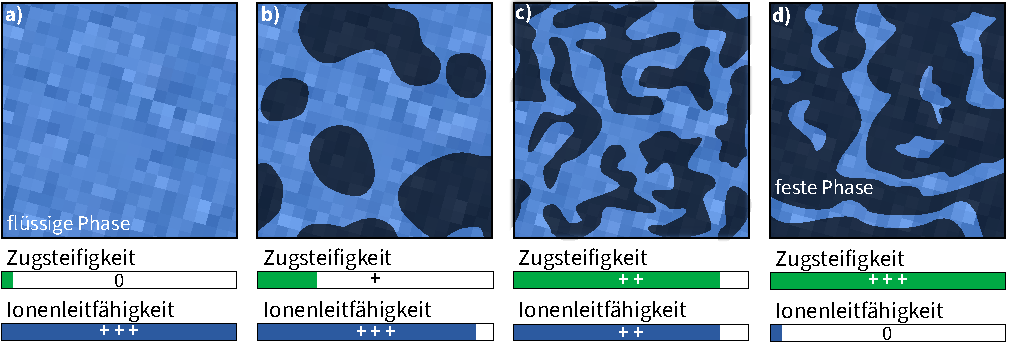
\includegraphics[width=\textwidth, angle=0]{bicontinous_electrolyte.pdf}
		\caption{\label{fig:bicontinous_electrolyte}Verännderung der Zugsteifigkeit und der Ionenleitfähigkeit mit zunehmenden festem Phasenanteil bei zweiphasigen Elektrolyten (a-d).}
\end{figure}
Zweiphasige Elektrolyte bestehen aus einer festen Phase, die für die mechansichen Eigenschaften verantwortlich ist, und einer flüssigen oder gelförmigen Phase, die für die Leitung der Ionen zuständig ist~\cite{Ichino1995}. Durch die Einstellung des Phasenanteils und der Kontrolle der Porenarchitektur kann können die resultierenden Eigenschaften zwischen den maximaler Leitfähigkeit und keinen mechanischen Eigenschaften und anderherum eingestellt werden, siehe Bild~\ref{fig:bicontinous_electrolyte}. In simualtiven Studien wurde mögliche idealen Architekturen und Phasenanteile zur maximalen Steigerung der Multifunktionalität bereits bestimmt~\cite{Lee2019,Tu2020}. Jedoch gibt es bisher nur eine bekannte Studie diese Nanostrukturen mithilfe von 3D-Druck zu fertigen~\cite{Zekoll2018}, jedoch mit $2,7 \times 10^4$ $\si{\milli  \siemens \per \cm}$ nicht den erklärten Grenzwert überschreiten konnte. Der exitierende Stand der Technik konzentriert sich daher hauptsächlich auf die Fertigung relativ ungeordneter Strukturen. Bei der Wahl des Phasenanteils sind dabei auch Untersuchungen aus der Percolations Theorie, die sich mit der Bildung von weitreichenden Verbunden in zufälligen Systemen beschäftigt, zu beachten. Untersuchungen mit zufällig angeordneten Kugeln zeigen, dass das bei 29,02~\% an leitender Phase erst ein Grenzwert überschritten wird bei dem eine durgehende Verbindung und damit eine Möglichkeit des Transportes von Ionen von einer Elektrode zur Anderen sichergestellt werden kann~\cite{Li2020b}. Die selbe Studie zeigt auch, dass durch Abweichung von der spherischen Struktur dieser Anteil auf 22,94~\% reduziert werden kann. Mit der Percolations Theorie ist somit ein wichtiges Mittel bei der Untersuchung des Verhaltens von zweiphasigen Elektrolyten und zum Beispiel erklärungsansätze warum bei bestimmten Anteilen von flüssiger Phase scheinbar plötzlich eine Steigerung von mehrern größen Ordnungen an Ionenleitfähigkeit beobachtet wird~\cite{Melodia2023}.
Für die feste Phase haben sich auf Harz basierte System hauptsächlcih wegen ihrer einfacheren Löslichkeit und damit kleineren Porenbildung durchgesetzt. Jedoch treten vermehrt Thermoplastische System in den Vordergurnd. Diese sind leichter in den Fertigungsprozess zu integrieren und bieten einen zusätzliche Sicherheit bei auftretenden Kurzschluss, da bei der auftretenden Wärmebildung der Thermoplast schmilzt und die Poren verschließt, was einen weiteren Ladungsaustausch unterbindet.
Als Ausgangsmaterialien für die flüssige Phase kommen ionische Flüssigkeiten~\cite{Huang2022,Shirshova2013,Wendong2021,Shirshova2014,Dzienia2020}, Lithiumsatzlösungen in orgischen Lösern~\cite{Gienger2015,Sakakibara2017}, ihre Kombination~\cite{Shirshova2014,Yu2016} und andere System~\cite{Feng2017} in betracht.


Feststoffelektrolyten bestehen beist aus einer Polymermatrix mit felxiblen Ketten um die Bewegung eines gelösten Salzes zu ermöglichen. Der Hauptvorteil an diesem Ansatz liegt in dem Verzicht auf flüchtige oder brennbare Bestandteilen und denen durch den Polymer bestimmten vergleichsweise guten mechansichen Eigenschaften. Allerdings ist die ionische Leitfähigkeit bei Raumtemperatur deutlich geringer als bei zweiphasigen Vertretern. Die Herstellung von Feststoffelektrolyten kann auf zwei Wegen erfolgen. Eine Möglichkeit stellt dabei die Polymerisation in Anwesenheit von Lithiumsalz dar. \textsc{Snyder et al.}~\cite{Snyder2007, Snyder2009} erreichte mit diesem Ansatz Ionenleitfähigkeiten von $1,6 \times 10^{-5}$ - $1,7 \times 10^{-3}$ $\si{\milli \siemens \per \cm}$ und damit verbunde Zugmodule von 552 bis 15~$\si{\MPa}$. Der zweite, häufigere benutzte, Ansatz nutzt eine Mischung von Polymeren mit Lithiumsalz. Für diese komplet festen zweiphasigen Elektrolytesysteme kommen häufig Epoxid~\cite{Matsumoto2011,Munoz2021,Wang2020b} oder PEO~\cite{Moreno2011,Ji2010,Guo2021} zum Einsatz.


\subsection{Separator}

\begin{table}[h!]
    \caption{Properties of different types of separators}
    \label{tab_separator_comp}
    %\begin{adjustwidth}{-\extralength}{0cm}
    \newcolumntype{C}[1]{>{\hsize=#1\hsize\centering\arraybackslash}X}%
    \begin{tabularx}{\textwidth}{
    %C{0.6}
    C{1} 
    C{1.8} 
    C{0.8} 
    C{0.8} 
    C{0.8} 
    C{0.6}
    }
        \toprule
        \textbf{Separatortyp}
        &\textbf{Separatormaterial} 
        &\textbf{Ionische Leit- fähigkeit\textsuperscript{*} (mS/cm)} 
        &\textbf{Zug- steifigkeit\textsuperscript{*} (GPa)}
        & \textbf{Festigkeit\textsuperscript{*} (MPa)}
        &\textbf{Ref.} \\
        \midrule
        %\legendsep{c0}&
        Glassfaser&Glassfaser&1.13&21
        &325
        &\cite{Deka2017}\\
        %\midrule
        \addlinespace
        %\legendsep{c10}&
        Polymer&RF/PLA&110&0.3271
        &15.2
        &\cite{Vargun2020}\\
        %\midrule
        \addlinespace
        %Gel polymer electrolyte&$\mathrm{PVA/KOH/K_3[Fe(CN)_6]}$&45.56&n.a.&n.a.&\cite{maHighPerformanceSolidstate2014}\\
        %%\midrule
        %\legendsep{c4}&
        Feststoff- elektrolyt&$\mathrm{PEGDGE/TETA/EMIBF_4}$&0.2&26
        &350
        &\cite{Hubert2022, Choi2022}\\
        %\midrule
        \addlinespace
        %\multirowcell{2}{\legendsep{c6}}&
        \multirowcell{2}{Keramik}
            &$\mathrm{PVDF/PPG/LiCl/CaTiO_3}$&n.a.&1.2
            &65
            &\cite{Alvarez‐Sanchez2019}\\
            &$\mathrm{PVB/Al_2O_3NW}$&13.5&n.a.
            &30
            &\cite{Liu2020a}\\
        %\midrule
        \addlinespace
        %Diode-like polymer electrolyte&PVP/PEI/SWCNT&n.a.&n.a.&n.a.&\cite{chowdhurySupercapacitorsElectricalGates2019}\\
        %%\midrule
        %Ceramic&NPs/PTFE/SiC&n.a.&n.a.&1.3&\cite{qinCeramicBasedSeparatorHighTemperature2018,zhaoInorganicCeramicFiber2017}\\
        %%\midrule
        %Tree-leave&Quercus rubra&n.a.&n.a.&n.a.&\cite{chenTrashTreasureFallen2022,wangMechanicalCharacteristicsTypical2010}\\
        %%\midrule
        %Eggshell membrane&Eggshell membrane&3.8&n.a.&6.59&\cite{yuUsingEggshellMembrane2012}\\
        %%\midrule
        %\legendsep{c8}&
        Cellulose&MCC/AMIM-Cl&298.6&5.43
        &71.71
        &\cite{Ahankari2022, Xu2020}\\
        %%\midrule
        %Graphene oxide&Graphene oxide paper&n.a.&n.a.&n.a.&\cite{shulgaSupercapacitorsGrapheneOxide2015,comptonTuningMechanicalProperties2012}\\
        %%\midrule
        %Metal-organic framework&Metal-organic framework&n.a.&n.a.&n.a.&\cite{mengMetalOrganicFrameworks2015,bundschuhMechanicalPropertiesMetalorganic2012}\\
        \bottomrule
    \end{tabularx}
    %\end{adjustwidth}
    \noindent{\footnotesize{\textsuperscript{*} The abbreviation not available (n.a.) is used.}}
\end{table}

\subsection{Pouchfolie}
Herkömmliche Pouchzellen sind mit einer kunststoffbeschichteten Aluminiumhülle vor Umwelteinflüssen geschützt. Insbesondere verhindert diese das Feuchtigkeit in die Batterie eindringt und giftige oder brennbare Stoffe aus der Batterie entweichen können. Außerdem ermöglichen die guten mechanischen und Wärmeleiteigenschaften der Alumiumfolie eine geringe Gesamtmasse und eine effizientere Temperaturregulierung der Zellen. Eine zunehmend wichtiger werdende Aufgabe, die allerdings noch nicht hinreichend erfüllt, wird ist das Aufbirngen einen äußeren Zelldruckes.
In mehrere Studien konnte gezeigt werden, dass durch einen hohen externen Druck die Kontaktierung zwischen Elektrode und Elektrolyte verbessert wird, was einen besseren Ionen- und Elektronentransport bewirkt. Außerdem können ungewünschte Nebenreaktionen unterdrückt werden, wie etwa Gasbildung und Dendritwachstum, was den Lithiumverlust beim Laden und Entladen reduziert und somit dem Kapazitätsverlust entgegenwirkt und das Batterieleben verlängert \cite{Mussa2018,Mueller2019,Sakamoto2019}.
Besonders Batterien mit Feststoffelektrolyten benötigen einen deutlich höherer Druck um den Kontakt zwischen Elektrode und Elektrolyte zu gewährleisten \cite{Boaretto2021}. Jedoch existiert zurzeit noch keine zufriedenstellende Lösung. Zwar wird bereits bei der Herstellung mittels verpressen der Elektroden ein gewisser Druck realisiert, allerdings können größere Drücke damit nicht appliziert werden oder über längere Zeit aufrechterhalten werden \cite{Garayt2023}. Daher wird oft versucht durch eine externen Einspannung auf Systemebene diesen Druck aufzubringen. Jedoch entsteht durch die innere Reibung der Batterien kein gleichmäßiger Druckverlauf, was dazuführt, dass äußere Zellen stärker belastet werden und weiter innen liegende Zellen kaum von dem äußeren Druck profitieren. Auch haben höhere Ausgleichsdrücke, dass Problem, dass diese eine höhere Anstrengung für das Gesamtpaket darstellen, was zu dickeren Materialien und damit einer niedrigeren Gesamtenergiedichte führt.
Einzig die Knopfzellen, die durch eine integrierte Feder einen definierten Druck auf eine, im Verhältnis zur Pouchzelle, deutlich kleinere Fläche auswirkt ist die einzige bekannte Lösung zu diesem Problem. Hinzukommt, dass auch hier der Massenanteil von Gehäuse zu Zelle deutliche höher ist als bei Pouchzellen.

Für Strukturbatterien sind bisher keine Alternativen zum herkömmlichen Aluminiumpouchfolie untersucht wurden \cite{Ye2024}. Jedoch gibt es viele Gruppen die ihre Strukturbatterien mit Pouchfolie zusätzlich in einen kohlefaserverstärkten Kunststoff einbetten \cite{Pattarakunnan2020,Asp2021}. 


\section{Aktuelle Ansätze zur Entwicklung und Auslegung von Strukturbatterien}

\section{Ungelöste Herausforderungen in der Entwicklung von Strukturbatterien}
Erstellung Bild siehe Kommentar in .tex Datei
%Bild in Inkscape erzeugt und als SVG sowie pdf_tex speichern (Speichern unter -> .pdf -> Text in PDF weglassen und LaTex Datei erstellen). 


\begin{figure}[h]
	%\raggedleft
		%\def\svgwidth{\columnwidth}
	\def\svgscale{0.98}
		\input{testbild.pdf_tex} 
		\caption{\label{fig:testbild}Testbild erzeugt mit Inkscape}
\end{figure}

Bild \ref{fig:testbild} %\cite{Dannemann.Kucher_et.al_AppliedSciences_2018}  

Verwendung Package SIUNITX %(siehe Datei latex_package_readme_siunitx.pdf)   

Anzugsdrehmoment von $M_{\textnormal{a}}=\SI{1.1}{\newtonmetre}$

von \SI{1}{\kilo\hertz} bis \SI{15}{\kilo\hertz}

mittlere Temperaturänderung von $\left\langle \Delta T_{\textnormal{p}}\right\rangle(t)<\SI{0.5}{\degreeCelsius}$

Masse von $m_{\textnormal{p}}=\SI[separate-uncertainty]{0.884 (15)}{\gram}$

(siehe Abschnitt \ref{ch:anhang})